\documentclass[a4paper, 12pt, oneside]{book} % Here you chose the paper size and font size. Te command onside ensures that pages are not shifted left and right (as is common for printed books). 
\usepackage[utf8]{inputenc} % Added to manage special characters, like Norwegian letters
\usepackage[T1]{fontenc} % To manage special characters
\usepackage[Lenny]{fncychap} % fancy chapter style (many more available, like Sonny, Bjarne, etc)
\ChNameVar{\Large\rm\bfseries} % Set name to serif, bold
\usepackage{fancyhdr} %to customize the headers
\fancyhead{\nouppercase}
%\usepackage[lmargin=1in, rmargin=1in, tmargin=1.5in, bmargin=1.3in]{geometry} %sets the margins for the pages
\setcounter{tocdepth}{2} %table of contents number depth for subsections (2 = x.x.x)
\setcounter{secnumdepth}{4} %numbering depth for headers for subsections in the text(4 = x.x.x.x)
\usepackage{url} %to include urls
\usepackage{lipsum}
\usepackage{listings} %include this if you want to include code in the thesis
\usepackage{amsmath,amssymb} %mathematical package
\usepackage[per-mode=symbol]{siunitx} %includes SI-units
\usepackage[bf]{caption} %makes float captions bold
\usepackage{array, booktabs} %to make better tables
\usepackage{graphicx} %to include graphics
\usepackage{float} %to include floats
\usepackage[export]{adjustbox} %to adjust floats
\usepackage{subfig} %to include subfigures
\usepackage{chngcntr} %will make it possible to change the counter for tables, figures etc. such as below
%\counterwithin{figure}{section} %change counter for figures within sections (also possible to choose for each chapter
%\counterwithin{table}{section} %change counter for tables within sections
\usepackage{color, xcolor} %edit e.g. text colors
\usepackage{hyperref} %Adding internal links in you document
\usepackage{bookmark}
\hypersetup{
    colorlinks,
    citecolor=black,
    filecolor=black,
    linkcolor=black,
    urlcolor=black
}

% Here you can customize the look of your citations and bibliography
\usepackage[backend = biber,
            natbib = true, % Adding the natbib style. This will enable the use of \citet and \citep
            style = authoryear, % This can be changed to numerical if you only want numbers
            maxcitenames = 2,   % max number of names to include before et. al.
            ]{biblatex}
% Declare the bibliography resource
% (which you might want to connect to
% for example Zotero)
\addbibresource{bibliography.bib}
\usepackage{comment} %to be able to comment out sections in the .tex files
\usepackage{afterpage} %to customize page commands such as below
\usepackage[version=4]{mhchem} %Package for chemical notation
\newcommand\myemptypage{
    \null
    \thispagestyle{empty}
    \addtocounter{page}{-1}
    \newpage
    } %sets new page command to insert an empty page without adding to the page counter or having a page number




\begin{document}
%%%%%%%%%%%%%%%%%%%%%%%%%%%%%%%%%%%%%%%%%%%%%%%%%%%%%%%%
%\begin{comment}
% The title page:
% For NTNU students this page will be generated automatically when submitting your paper, and should not be included in the final file from Latex. Delete or comment out the title page setup. The final report should then start with the first page being the abstract. I have included a title page here so it is possible to see how it may look like, and for those who does not get an automatically generated title page. Of course you will need to change the names and titles etc. to your case.

%the title page should be an odd page (right hand side)

\begin{titlepage}
\vspace*{1.5cm}

\noindent  \textcolor{gray}{\large Pau Verdeguer Blom-Dahl} \\
\vspace{1cm}

\noindent \textbf{\Large Interaction of High-Energy Gamma Radiation in the Active Galactic Nucleus of NGC 1068} \\
\vspace{0.5cm}

\noindent {\large A Theoretical and Computational Study.} \\



\vspace{7cm}
\noindent Physics Project\\
Supervisor: Michael Kacherließ \\
April 2025 \\

\vspace{0.2cm}
\noindent Norwegian University of Science and Technology \\
Faculty of Natural Sciences \\
Department of Physics \\

\begin{figure}[h]
    
\includegraphics[width=0.28\textwidth]{Figures/ntnu_basic.png}
\end{figure}
\end{titlepage}


% The pre-chapters
\chapter*{Abstract} %pre-chapters should not be numbered, hExploratoryence the "*"
\pagenumbering{roman} %introductory pages should be roman
\setcounter{page}{1}
\addcontentsline{toc}{chapter}{\protect\numberline{}Abstract} %add the chapter to the table of contents, this is not automatically added when creating unnumbered chapters (*). Add it in a chapter style, and keep all chapters on the same numberline indent regardless of number or not on the chapter
This is a combined template and guideline for writing your project. This template should give the structure and a couple of examples, and it should help you get started on the different chapters of your thesis. You can clone and use this document template (\LaTeX) for your report. You do not need to follow all the guidelines given here, use your own judgment. The idea behind this document is rather to give you a reference for how to set up your document, and what is common to include in the different parts. What follows in this abstract can serve as an example of what will be presented in the other parts too. More information on how to write \LaTeX is given in Chap.~\ref{chap:Theory}, so please go directly to that chapter if you have not written in \LaTeX before.

The abstract is a short summary of your work. It should give the reader enough information to grasp the content of your work and decide whether they want to read it. When you read journal papers, you will see that they are usually just a single paragraph long. For a thesis, the abstract can be somewhat longer, but you should make an effort to try to keep it short and condensed. In general, an abstract should answer most of these questions:
\begin{itemize}
\item Why is the motivation for this work? Why is the study useful?
\item What is the research question? What has been studied?
\item What is(are) the objective(s)?
\item What methodology was used? (What has been done/how was it done?)
\item What are the main results?
\item What are the main conclusions?
\end{itemize}

 %insert the chapter text from the files

%add an empty non-counted page by the command below in order to get the first chapter on the left hand side, if needed (check your page number so that the first chapter is on an odd page)


%%%%%%%%%%%%%%%%%%%%%%%%%%%%%%%%%%%%%%%%%%%%%%%%%%%%%%%%
%Customize the layout of the main content of your thesis

%\pagestyle{fancy} %set customized page style for header
%\fancyhf{} %clear header and footer fields
%\renewcommand{\headrulewidth}{0pt} %set to no rule
%\fancyhead[LE, RO]{\thepage} %set the page number at left for even, right for odd pages
%\fancyhead[RE, LO]{\leftmark} %set the chapter name at right for even, left for odd pages
%is is possible to design the header with the chapter as you wish, e.q. only the chapter or only the name, all lowercase instead etc.
%you could also design the footer if you wish, for example:
%\fancyfoot[LE, RO]{\thepage}
%\setlength{\headheight}{14.49998pt} %set the header height


%%%%%%%%%%%%%%%%%%%%%%%%%%%%%%%%%%%%%%%%%%%%%%%%%%%%%%%%
%main content 

\pagenumbering{arabic}

\chapter{Introduction}
\label{chap:Introduction}

In your introduction, it is common to start with a broad focus, and then narrow in. You could narrow in even further in the background section. The introduction section should give the perspective and background for your upcoming research question. This is where you can take an expansive and holistic view.

\section{Motivation}

It is common to have a motivation section in your introduction (it does not need to be singled out as a separate section though, your motivation could be just a part of your introduction). In this section, you should motivate your research question, which will come later. Why is your work interesting? Why is it important? What is the purpose and aim of this work? This motivation should lead toward the research question coming later.


\subsection{Research question}

The research question you are trying to answer through your thesis should be formulated in the introduction section. The purpose of the motivation should lead to a hypothesis, and the research questions should be formulated so that it can verify the hypothesis.

You can also formulate a set of objectives for your work to answer your research question.  It should be clear how these objectives together will answer your research question.

\section{Outline}

It is common to end the introduction with an outline of the thesis. Here you could briefly present the different chapters and their content.
\chapter{Active Galactic Nuclei}
\label{chap:Active Galactic Nuclei}
\section{General Concepts}
As technology progressed through the 20th century, astronomers were able to observe the universe in new ways, discovering new phenomena and objects that were previously unknown. Discoveries such as the cosmic microwave background and pulsars revolutionized our understanding of the universe and the laws of physics that govern it.

The third discovery which is often mentioned in the same breath as these two is that of Active Galactic Nuclei (AGN), or more precisely, quasars ("Quasi stellar radio sources").

These objects are among the most luminous and energetic in the universe, being able to outshine entire galaxies in a volume which is incredibly small. The energy output of these objects is so high that it is difficult to explain how they can produce so much energy. The most accepted theory is that this energy is produced by the accretion of matter onto supermassive black holes, which have masses ranging anywhere from $10^6$ to $10^{10}$ solar masses. The matter is heated up to millions of degrees, and the radiation produced is emitted across the electromagnetic spectrum through different processes.

The structure of AGNs is complex, with different regions emitting different types of radiation. Generally, we find the following \citep{RadiativeProcesses}:

\begin{itemize}
    \item \textbf{The Supermassive Black Hole:} A black hole whose origins are still debated, but which is believed to have formed in the early universe. It has a mass of $10^6 - 10^{10}$ solar masses, and is the source of the energy produced in AGNs.
    \item \textbf{The Accretion Disk:} A disk of matter orbiting the black hole, gradually being accreted onto it. The matter in the disk is heated to millions of degrees, emitting radiation across the electromagnetic spectrum.
    \item \textbf{The Corona:} A region of hot, ionized gas located beyond the accretion disk, believed to be the source of X-ray emission in AGNs.
    \item \textbf{The Obscuring Torus:} A region of dust and gas surrounding the accretion disk, which absorbs some of the radiation and re-emits it in the infrared.
    \item \textbf{The Broad Line Region:} A region of ionized gas composed of numerous small, rapidly moving clouds situated near the accretion disk. This region emits broad emission lines in the optical and ultraviolet spectrum due to the Doppler effect caused by the high velocities.
    \item \textbf{The Narrow Line Region:} A region of ionized gas located further away from the accretion disk, which emits narrow emission lines in the optical and ultraviolet spectrum. The narrowness of these lines is due to the lower velocities of the gas clouds.
    \item \textbf{The Jet:} Some AGNs present a region of highly energetic particles that are ejected from the poles of the black hole at relativistic speeds. These jets can extend for thousands of light-years and emit all kinds of radiation.
\end{itemize}

The figure below illustrates neatly the structure of an AGN.

\begin{figure}[H]
    \centering
    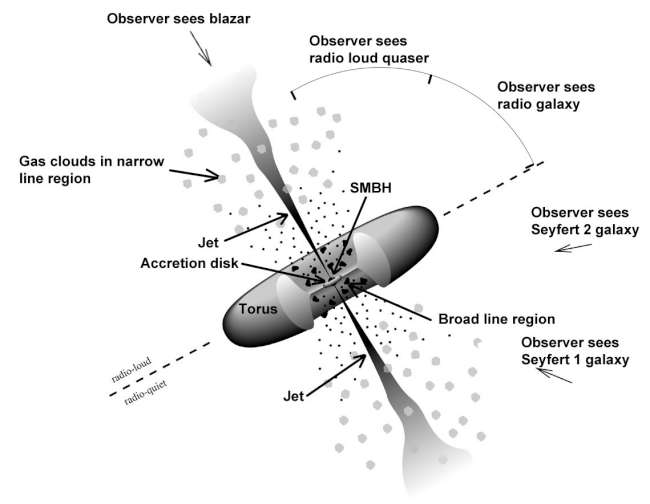
\includegraphics[width=0.7\textwidth]{Figures/AGN Structure.jpg}
    \caption{The structure of an Active Galactic Nucleus. The different regions mentioned before are labeled.}
    \label{fig:AGN_structure}
\end{figure}


\section{Radiation in AGNs}

The main topic of this project is the production of gamma rays in the AGN of NGC 1068, and how these gamma rays interact with the surrounding gas and radiation. We should first try to understand the underlying mechanisms that produce this type of radiation, as well as all the types of radiation at play in such regions.

It is also essential to make a distinction between thermal and non-thermal emission processes. Thermal emission has its origin in hot matter in the AGN. It follows a blackbody-like distribution, and is produced by particles which are in thermal equilibrium. Non-thermal emission, on the other hand, is produced by particles that are not in thermal equilibrium, and are accelerated to high energies, producing then radiation through different processes.

In general, AGNs emit radiation across the electromagnetic spectrum:

\begin{itemize}
    \item \textbf{Radio Emission:}
    \subitem \textbf{Synchrotron Radiation:} Generated by relativistic electrons spiraling in magnetic fields, which is common in AGN jets and lobes. In these sources the synchrotron spectrum typically covers photon energies from approximately $10^{-9}$ eV up to about $10^{-5}$ eV. In powerful radio-loud AGNs, this component can be extremely luminous, sometimes exceeding $10^{24}$ W Hz$^{-1}$.
    \subitem \textbf{Free-Free Emission:} Generated by the interaction of free electrons with ions in the gas, which is common in HII regions (regions of ionized hydrogen).
    \subitem \textbf{Maser Emission:} In some AGNs, molecules such as water in dense regions produce amplified microwave signals. This emission is typically observed around $10^{-6}$ eV and, while striking, generally represents only a minor fraction of the overall radio luminosity.
    
    \item \textbf{Infrared Emission:}
    \subitem \textbf{Thermal Dust Emission:} Dust in the circumnuclear torus absorbs high-energy photons and re-emits the energy in the infrared. The resulting spectrum covers energies from 0.001 to 1 eV. In obscured AGNs, this infrared component can dominate the bolometric output.
    
    \item \textbf{Optical/UV Emission:}
    \subitem \textbf{Thermal Emission:} The inner parts of the accretion disk surrounding the supermassive black hole are heated to temperatures high enough to emit thermal radiation that peaks in the optical/UV band. This emission typically spans photon energies from about 1 eV to 10 eV, and in many unobscured AGNs it is the dominant contributor to the total luminosity.
    \subitem \textbf{Broad and Narrow Line Emission:} In addition to the continuum, ionized gas in the broad-line and narrow-line regions produces characteristic spectral lines in the optical/UV. For example, the H$_{\alpha}$ line at 6563 \AA\ (about 1.89 eV) is prominent.
    
    \item \textbf{X-ray Emission:}
    \subitem \textbf{Non-thermal Emission:} Relativistic electrons in the jets can upscatter soft photons via inverse Compton scattering, producing X-rays typically in the range from 0.1 keV to 100 keV.
    
    \subitem \textbf{Bremsstrahlung:} In certain AGNs, collisions in the hot gas produce thermal X-ray emission, which generally occurs over a similar energy interval (roughly 0.1 - 100 keV). Although significant, this process usually contributes less to the total X-ray luminosity than the non-thermal component.
    
    \item \textbf{Gamma-ray Emission:}
    \subitem \textbf{Inverse Compton Scattering:} In the AGN jets, high-energy electrons collide with low-energy background photons, boosting them to gamma-ray energies. This mechanism typically yields gamma rays in the range of 100 keV up to more than 10 GeV, and in some blazars, it forms a major part of the high-energy emission.
    \subitem \textbf{Proton-Proton Interactions:} High-energy protons interacting with ambient protons can produce pions that decay into gamma rays (and neutrinos), often extending the spectrum into the TeV range (above $10^{12}$ eV). 
    \subitem \textbf{Proton-Photon Interactions:} Similarly, interactions between high-energy protons and low-energy photons lead to pion production and subsequent gamma-ray emission, further extending the high-energy tail into the TeV regime.
\end{itemize}


All in all, we get a complex distribution of energies in the AGN, with different processes producing different kinds of radiation. We can show this distribution in a spectral energy distribution (SED) plot, which shows the luminosity of the AGN as a function of frequency. Figure \ref{fig:AGN_SED} shows a schematic representation of the expected SED of a general AGN (excluding the radio and microwave bands, which are not shown).

\begin{figure}[h]
    \centering
    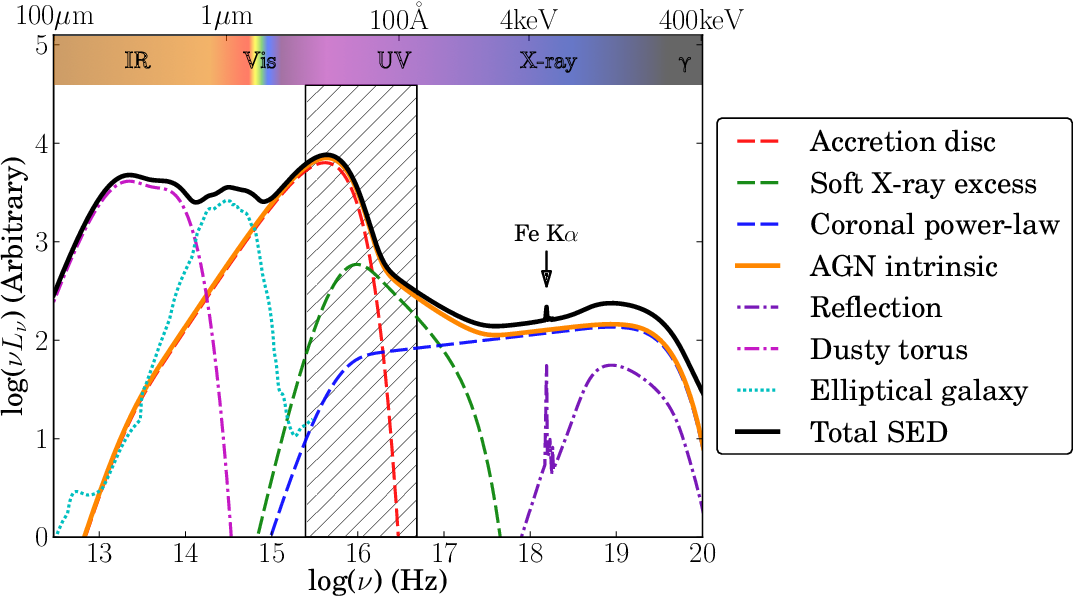
\includegraphics[width=\textwidth]{Figures/AGN SED.png}
    \caption{A simplified schematic diagram of an AGN SED, showing the approximate shape and extent of the various components discussed in the text. Dashed lines denote AGN intrinsic emission, dash-dot lines show emission reprocessed by the surrounding material and the dotted line shows starlight from an elliptical host galaxy. The hatched region highlights the spectral range that is heavily obscured by absorption in the IGM. We only show an elliptical galaxy here; galaxies with active star formation have stronger UV/IR contributions. Figure taken from \citet{QuasarSEDCollinson_2016}.}
    \label{fig:AGN_SED}
\end{figure}

Proton-proton interactions and proton-photon interactions in the AGN of NGC 1068 are of special interest, since these processes also produce neutrinos, whose energy spectrum is related to the gamma-ray spectrum in a clear and predictable manner.


\section{Gamma-ray Production in AGNs}

As mentioned above, gamma rays in AGNs are produced through different processes. We will focus on proton-proton and proton-photon interactions, which are sources of gamma rays and neutrinos in AGNs.

Inside AGNs, close to the supermassive black hole, we have a region of hot, ionized gas. This gas is composed of protons and electrons, which are accelerated to high energies by extremely high magnetic fields present in the region. These protons can then collide with other protons or photons in the gas, producing pions through the simplified processes specified below:


\begin{figure}[H]
    \centering
    \feynmandiagram [large, horizontal=a to b] {
        i1 [particle=\(p\)] -- [fermion] a,
        i2 [particle=\(\gamma\)]-- [photon] a,
        a -- c [blob, label=\(\Delta(1232)\)] -- b,
        b -- [fermion] f1 [particle=\(\pi^+_{(\nicefrac{1}{3})}\text{, }\pi^0_{(\nicefrac{2}{3})}\)],
        b -- [fermion] f2 [particle=\(n_{(\nicefrac{1}{3})}\text{, }p_{(\nicefrac{2}{3})}\)],
    };
    \caption{Proton-photon interaction.}
  \end{figure}

\begin{figure}[H]
  \centering
  \feynmandiagram [ large, horizontal=a to b] {
      i1 [particle=\(p\)] -- [fermion] a,
      i2 [particle=\(p\)]-- [fermion] a,
      a -- c [blob] -- b,
      b -- [fermion] f1 [particle=\(p\)],
      b -- [fermion] f2 [particle=\(n\text{, }p\)],
      b -- [fermion] f3 [particle = \(\pi^+\text{, }\pi^0\)],
  };
  \caption{Proton-proton interaction.}

\end{figure}

With the probabilites indicated as subindices. The pions produced then decay into gamma rays and neutrinos throught the following processes:
\vspace{-0.275cm}
\begin{figure}[H]
    \centering
    \begin{subfigure}{0.45\textwidth}
        \centering
        \feynmandiagram [medium, vertical=a to t1] {
            a [particle=\(\pi^{0}\)] -- [scalar] t1 [blob] -- [anti fermion, edge label'=\(k^-\)] t2 -- [anti fermion, edge label'=\(k^+\)] t3 -- [anti fermion, edge label'=\(k^+\)] t1,
            t2 -- [photon, blue] p1 [blue, particle=\(\gamma\)],
            t3 -- [photon, blue] p2 [blue, particle=\(\gamma\)],
            p1 -- [opacity=0] p2,
        };
        \caption{Neutral pion decay.}
    \end{subfigure}
    \begin{subfigure}{0.45\textwidth}
        \centering
        % Using the layered layout
        \feynmandiagram [layered layout, horizontal=k to b] {
        p [particle=\(\pi^{+}\)] -- [anti fermion] a [particle=\(\mu^{+}\)],
        p -- [red, fermion] d [red, particle=\(\nu_{\mu}\)],
        a  -- [anti fermion] b -- [red, anti fermion] f1 [red, particle=\(\overline \nu_{\mu}\)],
            b -- [boson, edge label'=\(W^{+}\)] c,
            c -- [red, fermion] f2 [red, particle=\(\nu_{e}\)],
            c -- [anti fermion] f3 [particle=\(e^{+}\)],
            };
        \caption{Charged pion decay.}
    \end{subfigure}
  \end{figure}

As you can see highlighted in blue and red, the pions decay into gamma rays and neutrinos, respectively.
The interesting part from this is that, since these particles come from the same source, it can be stated that a flux of neutrinos from the AGN of NGC 1068 is unavoidably accompained by a $\gamma$-ray flux $F_\gamma \sim 2 \times F_\nu$.

\section{The AGN of NGC 1068}

NGC 1068 is a Seyfert galaxy located in the constellation Cetus, approximately 47 million light-years away from Earth. It is one of the closest AGNs to our galaxy, and has been the subject of numerous studies due to its unique properties.

The publishing of data from the IceCube collaboration \citep{IceCube2022} has sparked numerous studies on the gamma-ray and neutrino emission from NGC 1068. Turning our attention to the SED of NGC 1068, we can see that the gamma-ray emission is expected to be comparable to the neutrino emission, as shown in figure \ref{fig:NGC1068_SED}.
\begin{figure}[H]
    \centering
    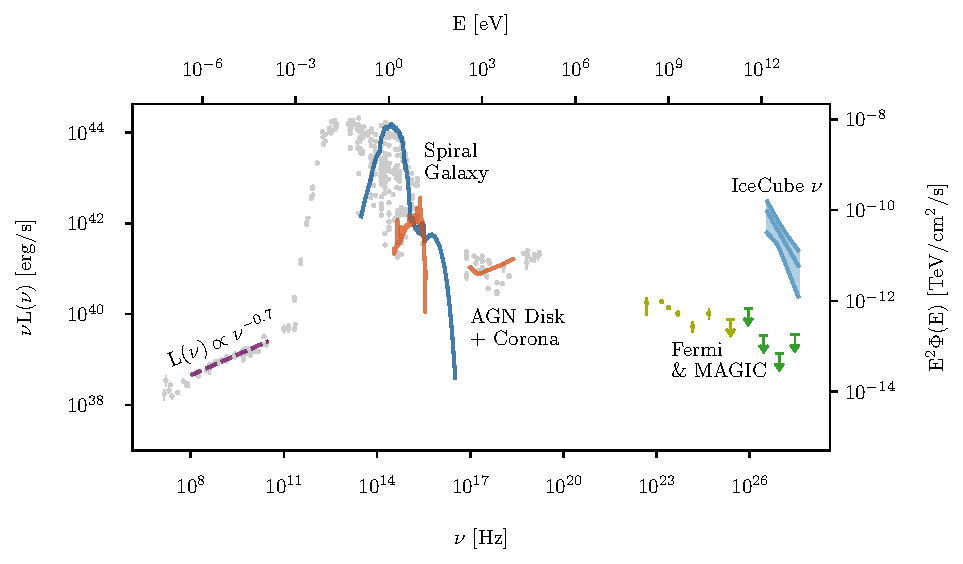
\includegraphics[width=0.7\textwidth]{Figures/NGC1068_SED.png}
    \caption{The SED of NGC 1068, showing the expected gamma-ray and neutrino emission.}
    \label{fig:NGC1068_SED}




%The background section should give sufficient background information to give the reader an overview of the state-of-the-art research field in which you work.

%The background chapter can be a bit similar to the introduction. For journal articles, it is not that common with a background section, as it is not kept separate from the introduction. However, for a master thesis, it is common to have more background and therefore to separate out some of the background material into a separate chapter. For a specialization project, the background chapter could be the most important chapter, as the specialization project is centered around learning a new subject field.

%Do not overestimate the background knowledge of the reader. As a rule of thumb, you could assume (s)he knows as much as you did when you started on your master thesis/project. So you need to give the reader enough background to be able to read the rest of your thesis.

%All relevant literature should be included, so do a thorough literature search. When you do, try not to miss out on the classics and defining papers in your field of work. For a specialization project, your background section can include references to display the breadth of the field you are working on. In contrast, for a master thesis, you should be able to argue for all included references. Do not add references just to get a long reference list. After you have spent a lot of time reading something, it could be tempting to add those references to just show off that you have read them, even though it turned out after reading them that it is not fully related to your work. Do not, all included references in your master thesis should be relevant to your work.

%The background material should also motivate your work. It should make your research question interesting by showing what others have done, and showing what is missing, highlighting the void that you try to fill with your work.


%\section{Citations}

%The background needs relevant literature to place your project work into context. The Google-scholar search (\url{scholar.google.com}) is a good starting point for searching for relevant papers.  This subsection will show how to include these references in your latex-document.

%There is a long range of different styles and packages in Latex for citations. During your writing process, it is often beneficial to have an \texttt{authoryear} style, where you see the author(s) and the year of publication. This will help you remember what the reference is. In the \texttt{main.tex} file you will find a command defining the bibliography style.

%This is where you want to go to change the style of your referencing. In this setup, we use the \texttt{natbib} style. This allows for using \verb=\citep= and \verb=\citet= references, which are useful if you use \texttt{authoryear} style:
%\begin{itemize}
 %   \item Whenever the reference is part of the sentence, you should use the textual citation \verb=\citet=. The \verb=\citet= reference types will give a reference that looks like this: \citet{berg2014permeability}.
 %   \item Whenever the reference is not a part of the sentence, but just general for the sentence or paragraph, you should use the parenthetical citation \verb=\citep=. The \verb=\citep= reference types will give a reference that looks like this: \citep{berg2014permeability}.
 %   \item If you do not specify, but use \verb=\cite=, it will look like this: \cite{berg2014permeability}.
%\end{itemize}

%All the references you use will automatically show up in your reference list. If you want to shift to numerical citations, you should use the \texttt{cite} command, as there are no differences between textual and parenthetical citations when you use the numerical style.
\chapter{Theory}
\label{chap:Theory}

The theory section is not as common to include as the other sections included in this document. Some work is theory-heavy, and it can be beneficial to split the theory part from the background and methodology parts of the document. In this document, we will rather use this section to show some important \LaTeX commands that you are likely to use.

When you write in \LaTeX, try to just follow the given style. You might not like the exact way of the given style in your document, but if you try to change it with small commands everywhere, you will probably end up with a document that looks worse, and you will spend a lot of time writing \LaTeX code in your document.

\section{Equations}

A simple equation or variable can be written within sentences using the dollar sign on each side, for example, writing \verb=$a$= will show up as $a$. The usual way of including an equation on a separate line is either by using double dollar signs, such as this:
$$E = mc^2$$
or using the \texttt{equation} environment:
\begin{equation}
    E=mc^2
    \label{eq:Einstein}
\end{equation}
\sloppy Note that the \texttt{equation} environment will enumerate the equation, and allow you to add a label that you can refer to later. When labeling the equations, you can refer to them using \verb=\eqref{<label>}=, which will give you an equation reference like Eq.~\eqref{eq:Einstein}.

The text below shows an example of how to align equations on the equal sign, with only one reference for both. This may be useful for when they are linked and are actually only one equation but splitting them up makes it more readable.
\begin{equation}
\begin{aligned}
        a &= \sin^{2}(\Delta\phi/2) + a \sin^{2}(\Delta\phi/2) \\
         &= (1+a) \sin^{2}(\Delta\phi/2)
\end{aligned}
\label{eq:splitTwoLines}
\end{equation}
The whole equation can be referenced as a single equation, Eq.~\eqref{eq:splitTwoLines}. One may also align sub-equations such that they are numbered the same but have a letter differentiating them as shown below\footnote{A footnote explaining something.}. This can be used when they are linked, but you will need to reference both individual parts.

\begin{subequations}
\begin{align}
    \sigma &= \sqrt{\frac{1}{N} \sum_{i=1}^N (x_i - \mu)^2}
    \label{eq:sd}\\ 
    \mu &= \frac{1}{N} \sum_{i=1}^N x_i \label{eq:mean}
\end{align}
\label{eqn:subeqn}
\end{subequations}\\
These equations can be referenced by their specific sub-equation as Eq.~\eqref{eq:sd}, or by the whole group as Eqs.~\eqref{eqn:subeqn}.


\section{Including figures}

Figure \ref{fig:qualityDiff} is an example of how to include figures in your \LaTeX document. This is also an example of the difference between a vector-based image format (pdf) and a voxel-based format (png). When possible, always try to use a vector-based image format, as that gives infinite resolution.

These two figures were created using this simple Python code:

\lstinputlisting[firstline=1, lastline=17,language=Python]{Figures/createPlot.py}

So when you create figures using Python, try to save them as pdf, as use the tight boundaries to save some space around the figures.

\begin{figure}[H]
  \centering
  \subfloat[Sinus figure using pdf.]{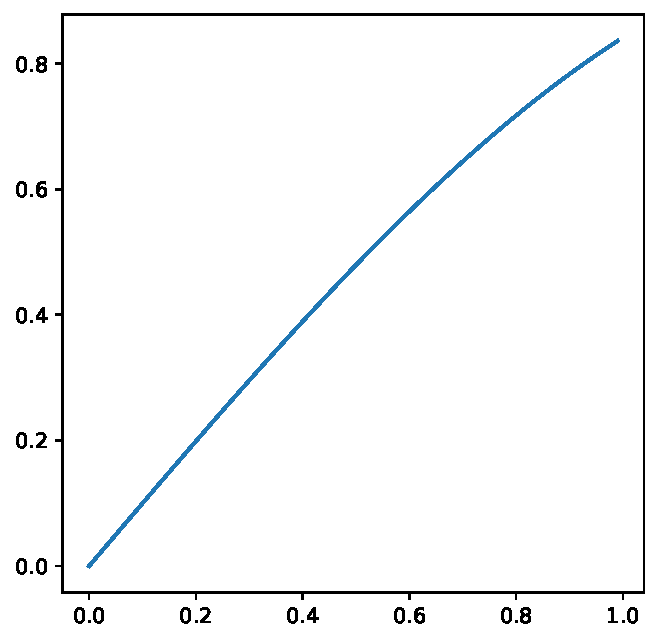
\includegraphics[width=0.45\textwidth]{Figures/sin.pdf}\label{fig:sinpdf}}
  \quad
  \subfloat[Sinus figures using png.]{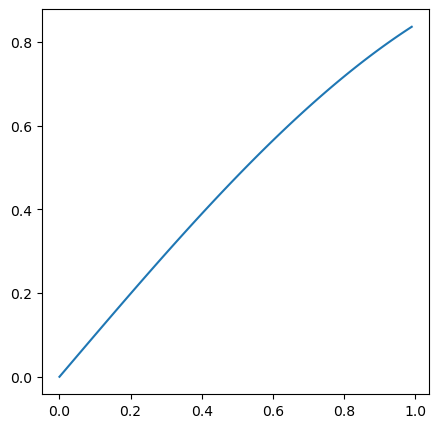
\includegraphics[width=0.45\textwidth]{Figures/sin.png}\label{fig:sinpng}}
  \caption{Figure (a) shows a pdf figure, while figure (b) shows a png figure. If you zoom in, you will start noticing the difference in quality.}
\label{fig:qualityDiff}
\end{figure}

With Python you could change the size of your figures. This is helpful for getting the right size of text within figures. In Figure \ref{fig:SizeDiff} we compare two different sizes.

\begin{figure}[H]
  \centering
  \subfloat[Sinus figure using size (8,8).]{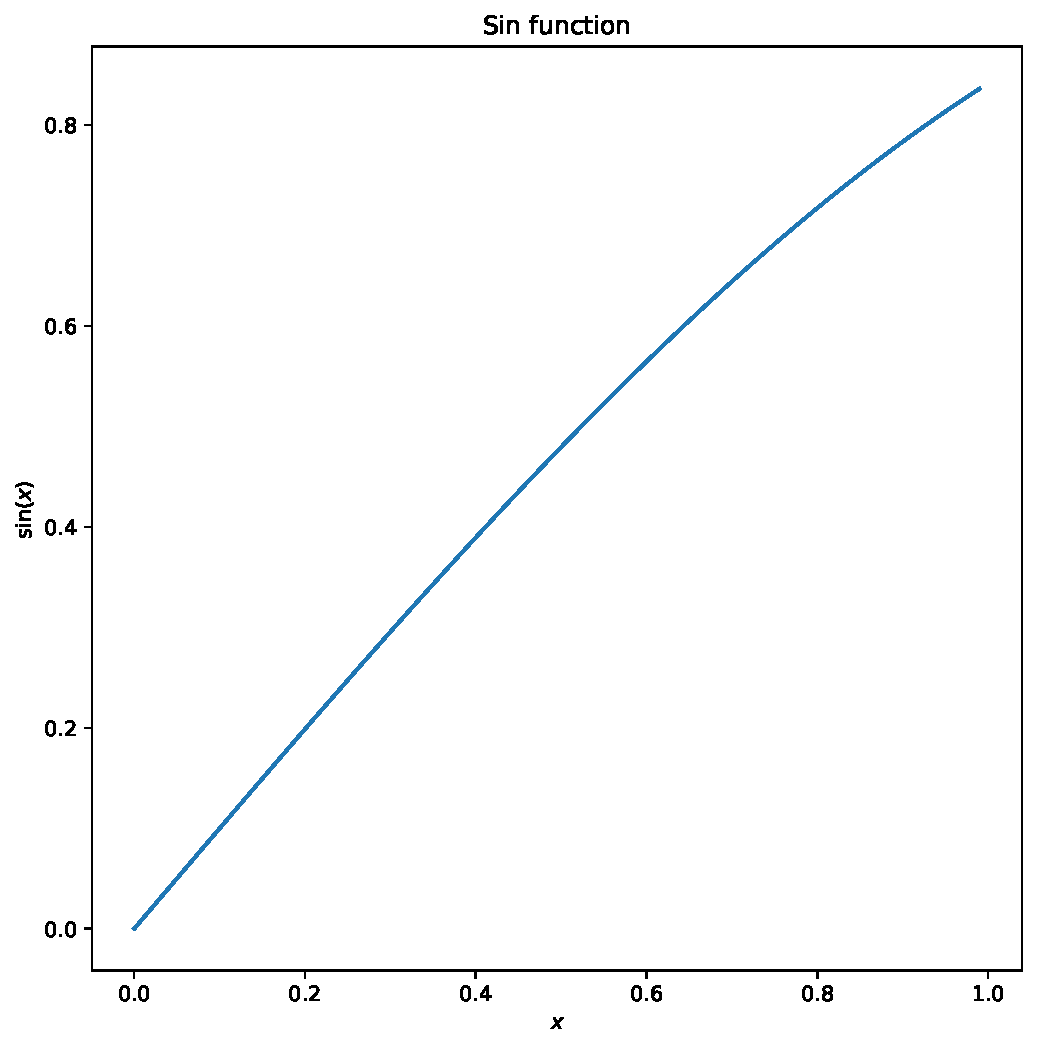
\includegraphics[width=0.45\textwidth]{Figures/sinBig.pdf}\label{fig:sinBig}}
  \quad
  \subfloat[Sinus figures using size (4,4).]{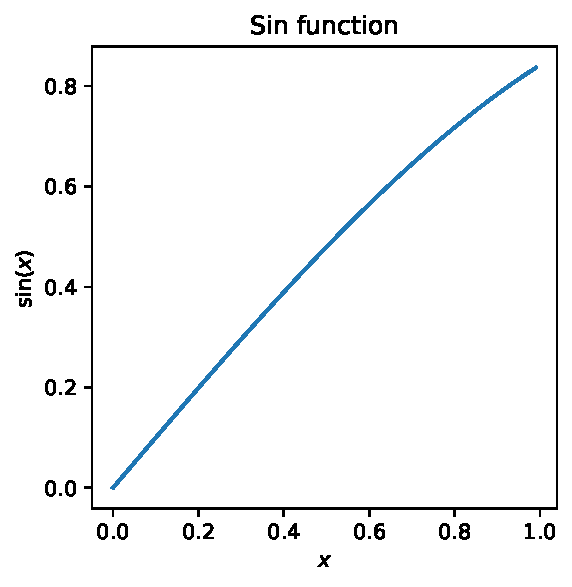
\includegraphics[width=0.45\textwidth]{Figures/sinSmall.pdf}\label{fig:sinSmall}}
  \caption{This is a comparison between two different figure sizes.}
\label{fig:SizeDiff}
\end{figure}


\section{Chemical notations and units}

This document has included a package for chemical symbols, \texttt{mchem}. When you write \verb=\ce{CO2}= you will get the chemical notation as \ce{CO2}.

For units we use the \texttt{siunitx} package. If you write \verb=\SI{10}{\meter\per\second\squared}= you get \SI{10}{\meter\per\second\squared}. The package can be used within math mode (inside the dollar signs). It automatically changes to a fixed notation for numbers, such as \verb=\SI{1E5}{\meter}= gives \SI{1E5}{\meter}.

\section{Tables}

Here are two examples of regular tables with data and a table with split headers.

\begin{table}[ht!]
\centering
    \begin{tabular}{ m{3cm} m{2.5cm} m{2.5cm} m{2.5cm} m{2cm} } 
    \toprule
    \toprule
    \textbf{Statistic} & \textbf{Velocity} & \textbf{Altitude} & \textbf{1/Angle} & \textbf{Temp.} \\
    \midrule
    Mean    & 122.68    & 240.98   & 93.75     & 13.95 \\[1.3ex]
    Std     & 224.51    & 145.88   & 60.39     & 4.44  \\[1.3ex]
    Q1      & 28.00     & 111.60   & 34.15     & 10.60 \\[1.3ex]
    Median  & 63.00     & 223.20   & 99.59     & 13.30 \\[1.3ex]
    Q3      & 137.00    & 359.10   & 151.99    & 16.70 \\[1.3ex]
    Min     & 0.00      & 1.00     & 0.00      & 3.30  \\[1.3ex]
    Max     & 14519.00  & 616.70   & 180.00    & 32.10 \\[1.3ex]
    \bottomrule
    \bottomrule
    \end{tabular}
% the square brackets after \caption gives the table a proper title in the list of tables, instead of just inserting the beginning of the table caption
\caption[Dynamic feature statistics with outliers]{Table of dynamic feature statistics where outliers are included, for all data points. Velocity is given in \textit{m/h}, the altitude in \textit{mamsl}, the inverse trajectory angle in 1/degrees, and temperature in degrees Celsius.}
\label{table:stat_fliers}
\end{table}


\begin{table}[ht!]
\centering
    \begin{tabular}{ m{3cm} m{5cm} m{3cm} } 
    \toprule
    \toprule
    \textbf{Area 1} & \textbf{Start date} & \textbf{End date} \\
    \midrule
    2018    & 03.06    & 29.06                       \\[1.3ex]
    2019    & 03.06    & 03.07 or 31.08\footnotemark \\[1.3ex]
    2020    & 03.06    & 05.09                       \\[1.3ex]
    \midrule
    \textbf{Area 2} & \textbf{Start date (farm 1/2)} & \textbf{End date} \\
    \midrule
    2012    & 09.06            & 07.09               \\[1.3ex]
    2013    & 23.06 / 15.06    & 25.08               \\[1.3ex]
    2014    & 05.06 / 25.06    & 10.09               \\[1.3ex]
    2015    & 13.06 / 03.07    & 06.09               \\[1.3ex]
    2016    & 17.06            & 22.07               \\[1.3ex]
    \bottomrule
    \bottomrule
    \end{tabular}
\caption[Selected time ranges for all data]{Selected time ranges for the data in all areas and all years.}
\label{table:time_ranges}
\end{table}

There are online tools to create \LaTeX tables. This might be a faster way of creating them than writing all the code yourself.

\chapter{Methods}

In this chapter, you describe the methods used to obtain your results. This can be new methods for analyzing existing data, or existing methods applied to new data. Include a complete description of your methods. It is often helpful with flow charts to explain your methods.

Give enough details for others to be able to reproduce your work. Do not overdo it, as a rule of thumb you can assume that the reader has the same background as you had when you started the thesis.

Introduce and describe all parameters that have been tested in your project, and why these in particular have been varied. What was the reason for varying these parameters?

Additional details can be given in the appendices. Appendices are useful to avoid too much information in the thesis itself, which can be detrimental to the reading experience.

If you are developing or using software, then it is common to include pseudo-codes for the software. The full code can be added as an appendix, but it is even better to upload the code to a public repository (e.g., \url{github.com}), and link the repository from the appendix.


\chapter{Results}
\label{chap:Results}

In this chapter, you describe the output from applying your methodology. Present your results in a clear manner, using a combination of figures and tables.

If you are doing lab experiments: What do you observe? Also include qualitative observations that might not be directly relevant (“we saw more production at the upper half of the core sample than the lower half, with most production leaving at the upper side-plane”).

If you are doing computations: What is the output from applying your code/software? Which part of your software is using the most computational power? How does it compare to other similar software?

Illustrate the results. Use graphs, images, and tables (see Chapter \ref{chap:Theory}).

A common challenge is to distinguish the results and the discussion section. Do not discuss your results in this chapter, that should be done in the discussion section. If it is hard to separate results and discussion, you might combine them into one section. You could also split the results and discussion part of your thesis into several results/discussion sections for different topics (“Magnesium effect on imbibition”, “Sodium effect on imbibition”).

Try to avoid repetition between. In case you have many graphs of the same process, keep some characteristic graphs and move the rest to an appendix. Then you describe one graph in detail and refer to the others in the appendix for changes between the results.
\chapter{Discussion}

In this chapter, you should expand on your results and address your main research questions (the research
questions were stated in Chapter \ref{chap:Introduction}). You should post-process and discuss the results already presented in Chapter \ref{chap:Results}.

What kind of information can you deduce based on the results you have compiled and presented in the Result section? How do the different results you have obtained compare to what you expected or to results reported by others? Cross-plot your results to extract information. Discuss variation between re-runs.

What do the results tell us? Try to answer your research questions. Provide the information you said you wanted to provide by conducting this study. Can you draw conclusions, and in particular, can you answer your research question? Can you give a negative answer? If not, is then a positive answer probable?
\chapter{Conclusions}

Give a concise summary of your research and findings here, and include a short summary of any future work as well.

You could also discuss the consequences and possible applications of your results. What does your result have to say for your scientific field? What are the economic consequences if your results are commercialized? What are the consequences for the society and environment?

\section{Future work}

Include a section about what should or could be done in future research, or explain any recommended next steps based on the results you got. This should be the last section of the conclusion chapter.

\addcontentsline{toc}{chapter}{\protect\numberline{}References}
\printbibliography[title={References}] % you may change the title in the toc here if you want
\cleardoublepage

\chapter*{\LARGE \textbf{Appendices}}
\fancyhf{} %clear the header, it should be empty for the appendices
\renewcommand{\headrulewidth}{0pt} %no rule
\fancyfoot[C]{\thepage} %set the page numbers in the center of the footer instead 

%it is possible to set a different page numbering style for the appendix, but I personally just continued with the same page numbering as the main content as I find that more tidy
%\pagenumbering{roman}
%\setcounter{page}{1}
\addcontentsline{toc}{chapter}{\protect\numberline{}Appendices:}
\appendix


\chapter*{A - Github repository}
\addcontentsline{toc}{chapter}{\protect\numberline{}A - Github repository} 

The MATLAB code utilized in this project can be found in the following repository:

\subsection*{Github repository link}
\begin{itemize}
    \item \url{https://github.com/Adelved/specialization-project}
\end{itemize}


%%%%%%%%%%%%%%%%%%%%%%%%%%%%%%%%%%%%%%%%%%%%%%%%%%%%%%%%



\end{document}
